Nella seguente sezione sono illustrati ed analizzati i dataset impiegati per il task di Sentiment Analysis nell'ambito delle news finanziarie. Ciascun dataset sarà composto da: una serie di news headline annotate con il relativo sentiment, che indicherà quanto il titolo finanziario in questione è appetibile da parte di un possibile investitore.

\subsection{FinancialPhraseBank}
Il primo dataset utilizzato allo scopo è stato preso dalla piattaforma Kaggle\footnote{\href{https://www.kaggle.com/datasets/ankurzing/sentiment-analysis-for-financial-news}{Kaggle dataset 1: FinancialPhraseBank}}. Si compone di 4846 news headlines annotate con tre classi (sentiment) e le classi sono rispettivamente positiva (28.1\% sul totale del dataset), negativa (12.5\%) e neutrale (59.4\%).

\begin{figure}[!ht]
    \centering
    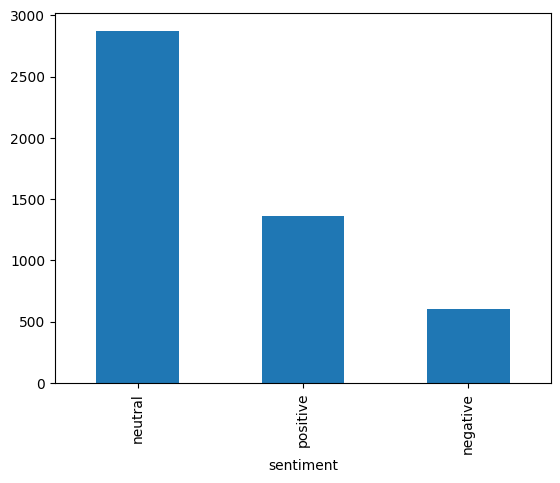
\includegraphics[width=10cm]{./images/dataset_percentage_bar_plot.png}
    \caption{Sample occurencies bar plot per class }
    \label{figure:dataset_perc}
\end{figure}

\subsection{FinancialPhraseBank + FiQA}
Il secondo dataset considerato per l'analisi è un estensione del precente, preso da Kaggle\footnote{\href{https://www.kaggle.com/datasets/sbhatti/financial-sentiment-analysis}{Kaggle dataset 2: FinancialPhraseBank + FiQA}}, che riporta in in totale 5322 news headline annotate nel medesimo modo del precedente dataset. 
Il dataset anche in questo caso si compone di tre classi e sono rispettivamente positiva (31.7\% sul totale del dataset), negativa (14.7\%) e neutrale (53.5\%). Il bilanciamento delle classi, a meno di piccole variazioni percentuali, è lo stesse del precedente dataset. \newline 
Indicate in Figure \ref{figure:dataset_perc}.

\newpage



